% kompiliert mit XeLaTeX
\documentclass{scrartcl}

% Deutsch, fontspec, microtype
\usepackage {polyglossia}
\setmainlanguage {english}
\usepackage {xltxtra}
\usepackage{microtype}

% Package für Bilder
\usepackage{graphicx}

% Mathe
\usepackage{amsmath, booktabs, hyperref}

% Kopfzeile
\usepackage{scrlayer-scrpage}
\pagestyle {scrheadings}
\rohead*{Kevin Lange\\Max Simon}

\begin{document}
	
	\part*{Exercise Sheet 03}	
	\section*{Part 2}
	For this exercise we used the provided \emph{tree.c} script. We implemented the algorithm also in Python (see \emph{tree\_alg.py}), which has a more detailed output and some functions to prove, if it works right, but because it is not optimized, it is very very slow.\\
	\\
	First of all, we were asked to calculate the moments of the current node from the subnodes moments. Because we use the monopole, it is sufficient to calculate the total mass of the node and the center of mass (\emph{calc\_multipole\_moments} function).\\
	\begin{align}
		M_\text{total} = \sum_{i = 0}^{7} m_i \quad m_i = \text{mass of subnode i}\\
		\vec{S} = \frac{\sum_{i = 0}^{7} m_i \cdot \vec{s}_i}{M_\text{total}}
	\end{align}
	Afterwards we were asked to calculate the acceleration on a particle out of the moments of the node (\emph{walk\_tree} function). From the lecture we know, that 
	\begin{equation}
		\phi(\vec{r}) = -G \cdot \left(\frac{M}{\vec{y}}\right), \quad \vec{y} = \vec{r} - \vec{s}
	\end{equation}
	Now one can calculate the acceleration by
	\begin{align}
		\ddot{\vec{r}} &= -\nabla \phi(\vec{r}) = - \frac{\partial \phi(\vec{r})}{\partial \vec{r}} = - \frac{\partial \phi (r)}{\partial \vec{y}} \frac{\partial\vec{y}}{\partial\vec{r}} = -\frac{\phi(\vec{r})}{\partial\vec{y}}\\
		&= G M \frac{\partial \left( y_1^2 + y_2^2 + y_3^2 \right)^{-0.5}}{\partial \vec{r}} = - \frac{G M \vec{y}}{| \vec{y} |^3}
	\end{align}
	So including the softening factor $\epsilon$ we get
	\begin{equation}
		\ddot{\vec{r}} = - \frac{G M \vec{y}}{[|\vec{y}|^2 + \epsilon^2]^\frac{3}{2}}
	\end{equation}
	We also implemented a counter into the function, to count, how many nodes got opened to calculate the acceleration for all particles (see \emph{counter} variable).\\
	\\
	The counter variable was also implemented in the \emph{main} function, where we added a loop for the exact calculation as well. The formula for the exact sumation was given in the lecture:
	\begin{equation}
		\ddot{\vec{r}}_i = −G \sum_{j = 0, j \neq i}^{N - 1} m_j \frac{\vec{r}_i −\vec{r}_j}{[(\vec{r_i} - \vec{r_j})^2 + \epsilon^2]^\frac{3}{2}} (\vec{r}_i - \vec{r}_j)
	\end{equation}
	Afterwards we added a calculation routine for the relative mean error $\eta$ given in the exercise. The script writes all important data (N, $\theta$, $t_\text{tree}$, Number of nodes per particle, $t_\text{exact}$ and $\eta$) to a file.\\
	\\
	The calculation is done with N = 5000, 10000, 20000 and 40000 for three $\theta$'s each: 0.2, 0.4 and 0.8. You can find all results in \autoref{results_ex_2}.\\
	There one can see, that $\eta$ is increasing with bigger values for $\theta$, but the calculation time decreases (only 1/4 if double $\theta$). The maximal mean error is always about 3\%, but can be decreased with a smaller $\theta$ to 0.1\%. The error seems to be independent of the number of particles.	
	\begin{figure}
		\centering
		\begin{tabular}{cccccc}
			\toprule
			N & $\theta$ & $t_\text{tree}$ [s] &  mean used nodes &  $t_\text{exact}$ [s] & $\eta_\text{mean}$ \\
			\midrule
			5000 &  0.200 & 1.64875 &  1736.48  &  6.8744 &  0.00128431 \\
			5000 & 0.400 & 0.467957 &  502.845 &  6.51361 &  0.00674545\\
			5000 & 0.800 & 0.103803  & 110.968  & 6.29948 & 0.0316469\\
			10000 & 0.200  & 4.73178  & 2404.89  & 25.1333 & 0.00145157\\
			10000 & 0.400  & 1.16883  & 622.909  & 25.1313 & 0.00698909\\
			10000 & 0.800 & 0.238019 &  128.757  & 25.1717 & 0.032126\\
			20000 & 0.200 &  13.9181  & 3121.22  & 104.066 & 0.001601\\
			20000 & 0.400 &  2.81475  & 738.402  & 104.437 & 0.00724406\\
			20000 & 0.800 & 0.553876 &  145.197  & 106.118 & 0.0320334\\
			40000 & 0.200 &  33.8408 &  3977.43 &  425.242 & 0.00168272\\
			40000 & 0.400 &  6.94127  & 867.969 &   425.35 & 0.00736282\\
			40000 & 0.800 &  1.28794 &  162.829 &  425.022 & 0.0323547\\
			\bottomrule
		\end{tabular}
		\caption{Results Exercise 2}
		\label{results_ex_2}
	\end{figure}
	
	\begin{figure}
		\centering
		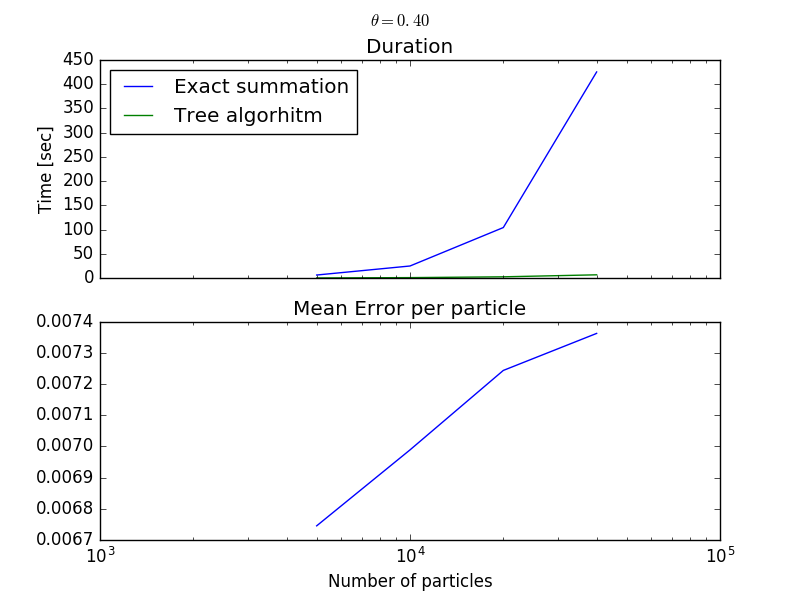
\includegraphics[width = \textwidth]{eval_th_4}
		\caption{Results for $\theta = 0.4$}
		\label{pic_1_ex_2}
	\end{figure}
	
	We plotted the calculation time for both methods in \autoref{pic_1_ex_2} as well as the mean error depending on N. One can see, that the calculation time for exact summation explodes, while the time for the tree method stays relatively small. The mean error is more or less linear (in the logarithmic scale!).\\
	\\
	To get an idea of the calculation time for $10^{10}$ particles, we used the approximations from the lecture:
	\begin{itemize}
		\item exact $\approx \alpha N^2$. Our data gave us a coefficient $\alpha = \frac{t_\text{exact}}{N^2} = 2.61 10^{-7}$ (mean value, relatively constant). So for $N = 10 ^{10}$ we would expect about 825000 years.
		\item tree $\approx \beta N \ln N$. Our data gave us a coefficient $\beta = \frac{t_\text{tree}}{N \ln N} =2.54 10^{-5}$ (mean value, differs about 10\%).So for $N = 10 ^{10}$ we would expect about 68 days.
	\end{itemize}
	From our estimates one can see, that for such large numbers only special algorithms like the tree algorithm can be applied. 
	
	
	
\end{document}